\documentclass[UTF8]{ctexbeamer}
\usepackage{hyperref}
\usetheme{Berlin}

\title{基本共射极放大电路的仿真与探究}
\author{薛昊辰,于宗玄,高浚哲,麻柯柯,胡潇丹}
\begin{document}
  
  \begin{frame}
    \maketitle
  \end{frame}

  \begin{frame}{摘要}
    本文详述了基本共射极放大电路的仿真结果,并结合当下背景,
对集成电路的应用进行了分析。
  \end{frame}

  \begin{frame}{电路原理}
    在整个共射极电路中,BJT为核心元件,起放大作用,输入电压Vs为BJT提供正偏电压,
并产生直流电流IB,直流电源Vcc为集电结提供反偏电压,使BJT工作于放大状态。
加入输入电压时,放大电路中的电流和电压既有直流成分也有交流成分,
所以在计算时要将交流与直流分开进行。
%\begin{figure}[h]
%    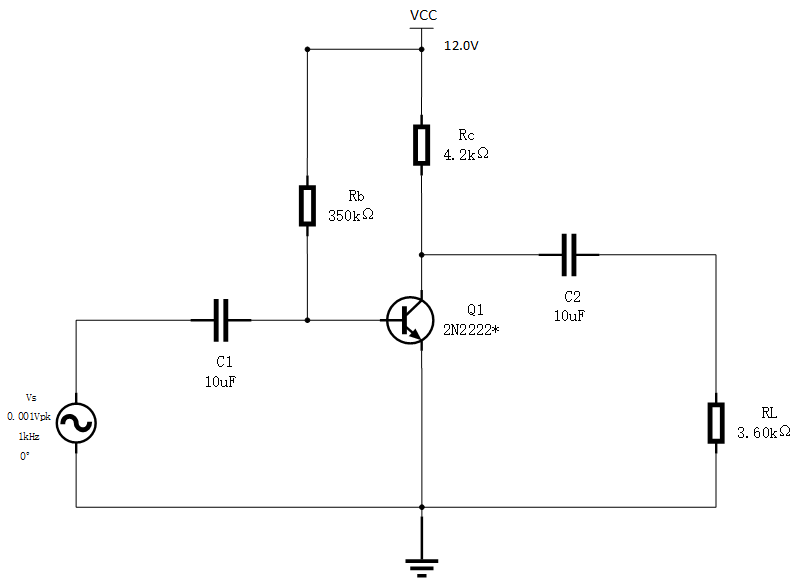
\includegraphics[width=8cm]{img/path1.png}
%    \caption{共射级放大电路}
%    %\label{共射级放大电路放大倍数测量}
%\end{figure}
  \end{frame}

  \begin{frame}{仿真计算过程}
    \textbf{元件选择}
    $10\mu f$电容2个,$4.2k\Omega$电阻1个,$3.6k\Omega$电阻1个,$350k\Omega$1个

    静态工作点理论值计算:

BJT基极电流
\begin{equation}
  \begin{split}
    I_{BQ}=\frac{V_{CC}-V_{BE}}{R_b}=\frac{12V-0.7V}{350k\Omega}=32.29\mu A
  \end{split}
\end{equation}

由BJT的分配电流关系求得BJT集电极电流
\begin{equation}
  I_{CQ}=\beta I_{BQ}=50\times32.29\mu A=1.615mA
\end{equation}

BJT射级电流
\begin{equation}
  I_{EQ}=(1+\beta)I_{BQ}=1.647mA
\end{equation}

  \end{frame}



\begin{frame}{仿真计算过程}
由电路结构可求得$V_{CEQ}$
\begin{equation}
  \begin{split}
    V_{CEQ}&=V_{CC}-I_{CQ}R_C\\
    &=12V-1.615mA\times 4.2k\Omega=5.217V
  \end{split}
\end{equation}

电压增益理论值计算:
\begin{equation}
  \begin{split}
    A_V&=\frac{V_o}{V_i}\\
    &=\frac{-\beta i_b(R_C//R_L)}{i_br_{be}}\\
    &=\frac{-\beta(R_C//R_L)}{r_{be}}=-96.6
  \end{split}
\end{equation}

\begin{equation}
  r_{be}=r_{bb'}+(1+\beta)\frac{26mV}{I_{EQ}}=1003.6\Omega
\end{equation}
\end{frame}

\begin{frame}{仿真计算过程}
\end{frame}

\begin{frame}{思政综述} 
    科学技术是第一生产力,
对于一个国家而言,要想在社会经济建设中获取更多的力量支撑,
就必须注重于自身科学技术水平的提升,
这是一个国家及社会进步的根本保障。
从当前的情况来看,电子信息技术较之前有了较大的进步与发展,
正逐渐的涉及到社会各个行业领域,给我们的生活方式带来极大的转变。
但是就因为其运用领域的宽阔性,不可避免的导致一些问题的发生。
因此,必须要从实际出发,针对这些问题做出分析,并采取可行的措施予以应对,
只有这样才可以确保我国电子信息技术水平的进一步提升。
\end{frame} 

\end{document}
